\chapter{Diseño e implementación} % Main chapter title

\label{Chapter3}

%----------------------------------------------------------------------------------------
%	SECTION 1
%----------------------------------------------------------------------------------------

-----------------------------------------------------------------------------------------
\section{Elementos componentes del sistema}
\label{sec:elementos_componentes_sistema}

%% - Breve descripcion de Firmwares y Bootloaders (software de vuelo)
%% - Descripcion de computadora a bordo
%% - Descripcion componentes a emular (Memoria RAM y microprocesador)

En el presente trabajo, no se ha modelado una memoria persistente, por lo que se ha agregado una función que recibe un archivo binario (FSW) y lo carga en la memoria RAM del sistema. Dicha funcion posicionará al binario en la dirección correcta de memoria, donde el CPU lo pueda ejecutar.

La figura \ref{fig:carga_binario} muestra un diagrama de flujo del procedimiento de carga y ejecución de un software en el emulador desarrollado. El diagrama asume que ya se posee un archivo binario valido para la arquitectura SPARC V8.

\begin{figure}[htbp]
	\centering
	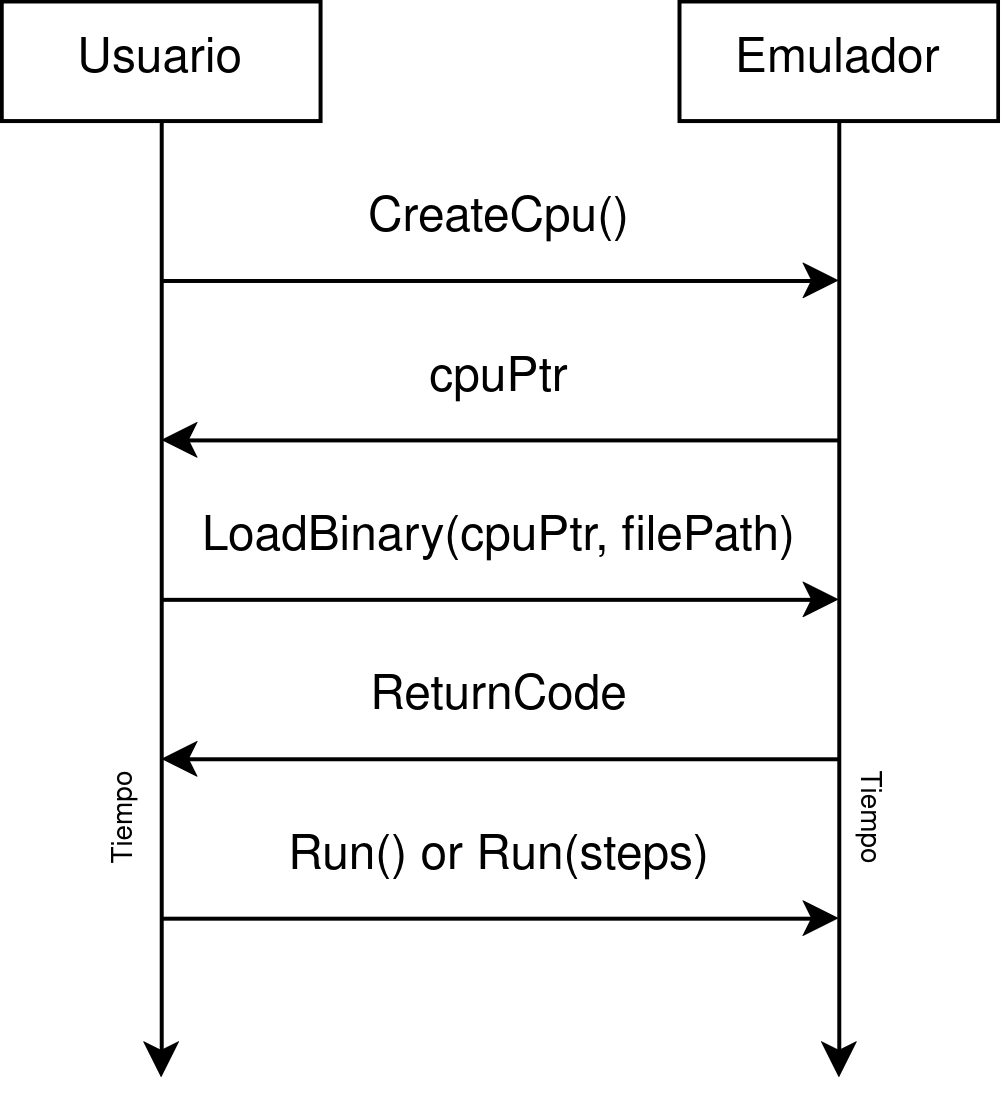
\includegraphics[width=.6\textwidth]{./Figures/carga_binario}
	\caption{Proceso de carga de binarios en emulador.}
	\label{fig:carga_binario}
\end{figure}

\newpage

Todo el procedimiento descrito anteriormente se lleva a cabo en la computadora a bordo (OBC) del sistema. La OBC es el componente que se encarga de orquestar el resto de los subsistemas del sistema. En un escenario real, la OBC tendría más componentes que los que se han modelado en este trabajo, tales como periféricos de comunicación UART, CAN y SpaceWire, entre otros. La figura \ref{fig:componentes_desarrollados}, tomada de la página de Gaisler \citep{GR712RC} y editada, muestra en detalle todos los componentes de la OBC GR712RC resaltando en rojo los componentes que se han modelado en el presente trabajo.


\begin{figure}[htbp]
	\centering
	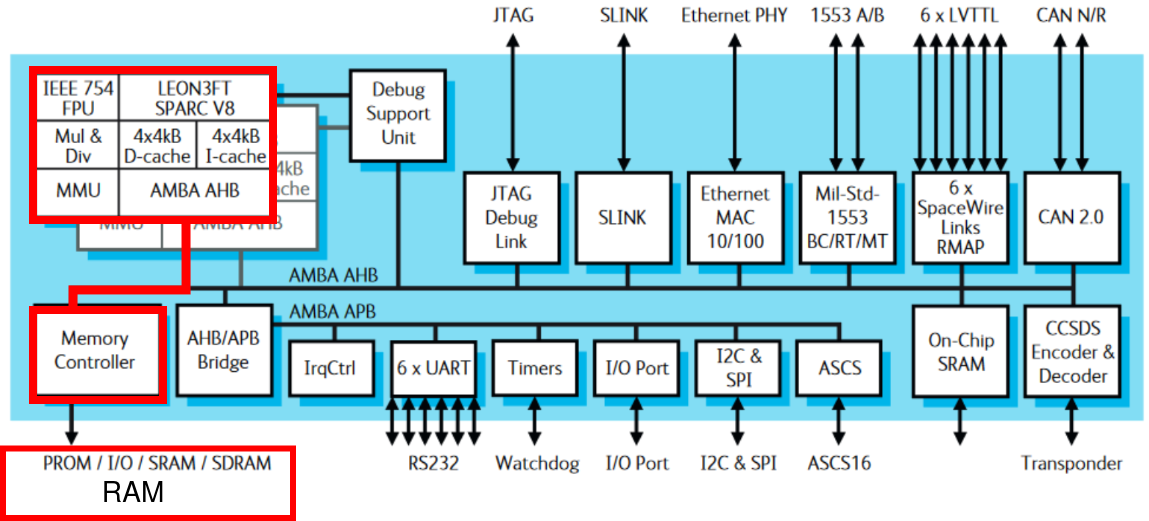
\includegraphics[width=1\textwidth]{./Figures/componentes_desarrollados}
	\caption{Componentes emulados.}
	\label{fig:componentes_desarrollados}
\end{figure}
\newpage

Cabe destacar que se utilizó la placa de desarrollo GR712RC como referencia para el desarrollo del emulador, ya que es una placa de desarrollo de uso común en aplicaciones espaciales. Se pueden destacar las siguientes simplificaciones realizadas:

\begin{itemize}
\item Se ha modelado únicamente un CPU. Esta simplificación permite omitir todas las instrucciones de sincronización y manejo de interrupciones que se deberían implementar en un sistema multi-core.
\item Se ha modelado el controlador de memoria (MCU por sus siglas en inglés \textit{Memory Controller Unit}) correctamente.
\item Las memorias PROM, I/O, SRAM y SDRAM se ha modelado como un único bloque de memoria RAM. Dicha simplificación reduce significativamente el número de modelos a implementar. Cabe aclarar que la presente simplificación no afecta el funcionamiento del emulador.
\end{itemize}


Para la CPU, se desarrollaron las siguientes instrucciones de la arquitectura SPARC V8:

\begin{enumerate}

\item \texttt{UNIMP}: Genera un interrupción de procesador.
\item \texttt{Bicc}: Salto condicional (Números enteros).
\item \texttt{SETHi}: Escritura de los 22bits mas significativos de un registro.
\item \texttt{FBfcc}: Salto condicional (Números punto flotante).
\item \texttt{CBfcc}: Salto condicional (Códigos de condición).

\item \texttt{CALL}: Llamada a subrutina.

\item \texttt{ADD}: Adición.
\item \texttt{ADDcc}: Adición con código de condición.
\item \texttt{ADDX}: Adición con retorno de carro.

\item \texttt{SUB}: Sustracción.
\item \texttt{SUBcc}: Sustracción con código de condición.
\item \texttt{SUBX}: Sustracción con retorno de carro.

\item \texttt{AND}: Operación \texttt{AND} lógica.
\item \texttt{ANDcc}: Operación \texttt{AND} lógica con actualización de código de condición.
\item \texttt{ANDN}: Operación de \texttt{AND} negada lógica.

\item \texttt{OR}: Operación \texttt{OR} lógica.
\item \texttt{XOR}: Operación de \textit{exclusive or}.
\item \texttt{ORcc}: Operación \texttt{OR} lógica con actualización de código de condición.

\item \texttt{SLL}: Desplazamiento lógico a la izquierda.
\item \texttt{SRL}: Desplazamiento lógico a la derecha.
\item \texttt{SRA}: Desplazamiento aritmético a la derecha.

\item \texttt{RDPSR}: Lectura del registro de estado del procesador.

\item \texttt{RDY\_RDASR}: Lectura del registro \texttt{Y} del procesador.

\item \texttt{WRY}: Escritura del registro \texttt{Y} del procesador.
\item \texttt{WRPSR}: Escritura del registro \texttt{PSR} del procesador.
\item \texttt{WRWIM}: Escritura del registro \texttt{WIM} del procesador.
\item \texttt{WRTBR}: Escritura del registro \texttt{TBR} del procesador.

\item \texttt{TICC}: Interrupción en código de condición de enteros.

\item \texttt{JMPL}: Salto incondicional.
\item \texttt{FLUSH}: Limpieza de operaciones pendientes.
\item \texttt{SAVE}: Guardado de ventana de procesamiento.
\item \texttt{RESTORE}: Carga de ventana de procesamiento.

\end{enumerate}


\section{Consideraciones y decisiones tecnicas}
\label{sec:consideraciones_decisiones_tecnicas}

Un desafío que se tuvo que resolver temprana en el desarrollo del emulador fue la endianess del sistema. El endianess es el orden en el que se almacenan los bytes en la memoria. En el caso de la arquitectura SPARC V8, se utiliza el ordenamiento \textit{big-endian}, lo que significa que el byte más significativo se almacena en la dirección de memoria más alta. Por otro lado, la arquitectura x86 (Es decir, nuestros computadoras de escritorio) utiliza el ordenamiento \textit{little-endian}, donde el byte menos significativo se almacena en la dirección de memoria más baja. Por lo tanto, al momento de interpretar los datos obtenidos de la memoria, se debe reordenar los bytes para que tengan sentido. Dicha problemática es propia únicamente del emulado

\section{Diagrama de bloques}
\label{sec:diag_bloques}

\section{Arquitectura del software}
\label{sec:arquitectura_software}

\section{Modulos componentes del software}
\label{sec:modulos_componentes_software}


\section{Desarrollo del software}
\label{sec:desarrollo_software}

